\documentclass[12pt, a4paper]{article}

\usepackage[czech]{babel}
\usepackage[IL2]{fontenc}
\usepackage[utf8]{inputenc}
\usepackage{lmodern}  % lepší kvalita PDF

\usepackage[a4paper,top=3cm,bottom=3cm,left=3cm,right=3cm,marginparwidth=1.75cm]{geometry}

\usepackage{graphicx}
\usepackage{titling}
\usepackage{enumitem}
\usepackage{caption}
\usepackage{float}
\usepackage{pdfpages}
\usepackage{verbatim}
\usepackage{amsmath}

\usepackage{listings}
\lstset{numbers=left,
	inputencoding=latin1,
	basicstyle=\scriptsize\ttfamily,
	keywordstyle=\color{blue},
	breaklines=true, 
	showtabs=false,
	showstringspaces=false,
	numberstyle=\tiny\color{gray},
}

\usepackage{multirow}

\usepackage{pkg-custom-commands}
\usepackage{pkg-url}


% údaje na titulní straně
\title{Samostatná práce}
\def \thesubtitle {KIV/PSI}
\author{Patrik Harag}
\def \theauthoremail {harag@students.zcu.cz}
\def \theauthorid {A18N0084P}

\begin{document}

\begin{titlepage}
	\begin{figure}
		
\includegraphics[height=50mm]{img-fav-logo}
	\end{figure}
	
	\centering
	{\large \hspace{1mm} \par} % tady musí být nějaký text jinak nefunguje vertikální odsazení
	\vspace{15ex}
	
	{\huge\bfseries \thetitle \par}
	\vspace{2ex}
	{\scshape\Large \thesubtitle \par}
	\vspace{15ex}
	{\Large\itshape \theauthor \par}
	\vspace{2ex}
	{\texttt{\theauthoremail} \par}
	\vspace{1ex}
	{\texttt{\theauthorid} \par}
	
	\vfill

	{\today\par}
\end{titlepage}


\section*{Zadání}
Protokol POP3


\section*{Analýza}
POP3 je textový protokol pro přístup k emailové schránce.
Je specifikován v RFC 1081\footnote{\url{https://tools.ietf.org/html/rfc1081}}.
Pracuje přes TCP/IP připojení užívající TCP port 110.
Případně může být přenášen přes SSL a využívat nejčastěji port 995.

\paragraph{Příkazy}
Protokol definuje několik příkazů: USER, PASS, STAT, DELE, RSET, QUIT, LIST, RETR.
Příkazy mají nejvýše jeden parametr, který je oddělen mezerou. Příkaz je zakončen sekvencí CR LF.

\paragraph{Odpovědi příkazů}
Za každým požadavkem musí následovat odpověď serveru. Kladná odpověď vždy začíná \code{+OK} a záporná \code{-ERR}. Následuje mezera a obsah sdělení.
Příkazy můžeme podle jejich odpovědí rozlišit na dva typy:
\begin{itemize}
	\item příkazy s jednořádkovou odpovědí (USER, PASS, STAT, DELE, RSET, QUIT),
	\item příkazy s víceřádkovou odpovědí (LIST, RETR).
\end{itemize}
Příkazy s víceřádkovou odpovědí jsou ukončeny řádkou se samotnou tečkou.
V případě, že je v obsahu zprávy na řádce samotná tečka, escapuje se tato tečka přidáním další tečky.

\paragraph{Typický scénář}
\begin{enumerate}
	\item Přihlášení
	\begin{enumerate}
		\item USER -- Zadá uživatelské jméno
		\item PASS -- Zadá heslo a pokusí se přihlásit
	\end{enumerate}
	\item Práce se schránkou
	\begin{itemize}
		\item STAT -- Informace o počtu zpráv a jejich celkové velikosti
		\item LIST -- Seznam zpráv
		\item RETR -- Vrátí zprávu ve formátu MIME\footnote{\url{https://en.wikipedia.org/wiki/MIME}}
		\item DELE -- Smaže zprávu
	\end{itemize}
	\item (Alternativní) Vrácení změn, zpět na krok 2 – RSET
	\item Odhlášení uživatele a potvrzení změn -- QUIT
\end{enumerate}


\section*{Implementace}
Byl implementován POP3 klient s uživatelským rozhraním, který umožňuje prohlížení zpráv a jejich mazání.
Pro implementaci byl zvolen programovací jazyk Java a framework JavaFX.
Pro parsování mailů ve formátu MIME byla použita knihovna Apache Commons Email. 
Program má následující strukturu:
\begin{itemize}
	\item \code{cz.harag.psi.sp} -- Obecné doménové třídy, hlavní logika, vstupní třída \code{Main}.
	\item \code{cz.harag.psi.sp.ui} -- Uživatelské rozhraní.
\end{itemize}

\paragraph{Nejdůležitěji doménové třídy}
\begin{itemize}
	\item \code{Connection} -- Rozhraní pro spojení.
	\item \code{SocketConnection} -- Implementace spojení pomocí socketů z \code{java.net}.
	\item \code{POP3Client} -- Poskytuje nízkoúrovňové API pro práci s POP3.
	\item \code{POP3ClientHelper} -- Poskytuje vysokoúrovňovější metody pro práci s POP3.
	\item \code{POP3Exception} -- Výjimka týkající se chyb v rámci POP3 protokolu.
\end{itemize}


\section*{Obsluha}

\paragraph{Kompilace a spuštění}
Program se zkompiluje spuštěním \code{build.bat} a spustí spuštěním \code{run.bat} (vyžaduje Javu 8).
Je použit Gradle, pro sestavení však není potřeba ho instalovat.

\paragraph{Ovládání}
Po spuštění aplikace se jako první zobrazí dialog se specifikací POP3 serveru, viz obrázek \ref{fig:gui-1}.
Po zadání údajů se zobrazí dialog pro přihlašovací údaje, viz obrázek \ref{fig:gui-2}.
Při zadání chybných přihlašovacích údajů se zobrazí chyboví dialog a řízení se vrátí zpět k přihlašovacímu dialogu.

\begin{figure}[H]
	\centering
	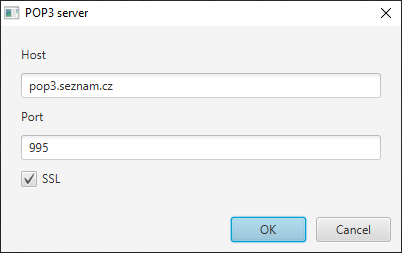
\includegraphics[width=0.6\linewidth]{gui-1}
	\caption{Dialog se specifikací serveru}
	\label{fig:gui-1}
\end{figure}

\begin{figure}[H]
	\centering
	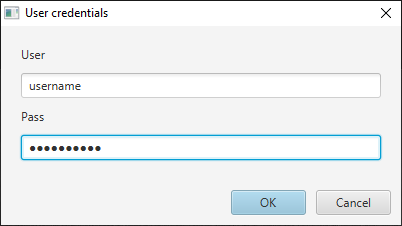
\includegraphics[width=0.65\linewidth]{gui-2}
	\caption{Dialog pro přihlašovací údaje}
	\label{fig:gui-2}
\end{figure}

\noindent
Při úspěšném přihlášení se zobrazí hlavní okno aplikace, viz \ref{fig:gui-3}.
Po výběru zprávy v levém panelu se její obsah zobrazí.
Integrovaný webový prohlížeč dokáže zobrazit i~HTML zprávy.
Zprávu je možné smazat přes kontextové menu v seznamu zpráv.

\begin{figure}[H]
	\centering
	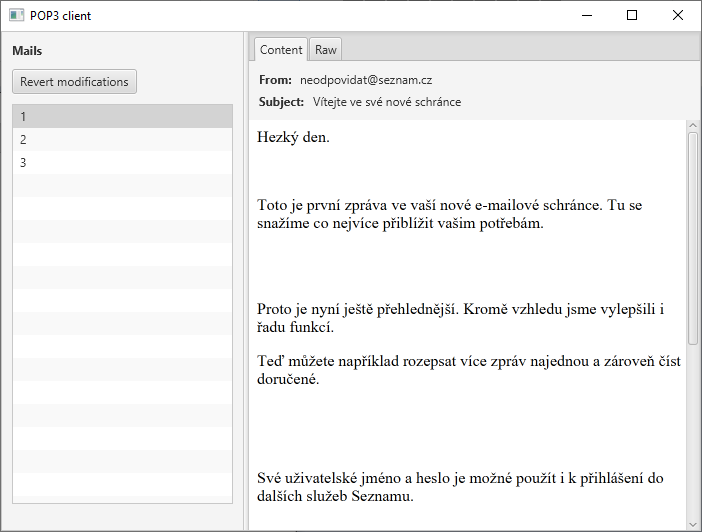
\includegraphics[width=1\linewidth]{gui-3}
	\caption{Hlavní okno aplikace}
	\label{fig:gui-3}
\end{figure}


\section*{Závěr}
Byl vytvořen POP3 klient s uživatelským rozhraním.
Aplikace při své činnosti vypisuje veškerou komunikaci s POP3 serverem, a tak může sloužit ke studijním účelům.
Aplikace byla otestována na reálném poštovním serveru \code{seznam.cz}.


% \bibliographystyle{plain}
% \bibliography{references}

% \chapter*{Přílohy}
% \section*{xxx}
% \lstinputlisting[label={xx}, caption={yy}]{sources.java}

\end{document}